\subsubsection{Financial Data Structures}

Four essential types of financial data
\begin{flushleft}
\begin{tabularx}{\textwidth}{X|X|p{13em}|X}
\hline
\rowcolor{gray!30}
Fundamental Data & Market Data & Analytics & Alternative Data \\
\hline
\xxx Assets 
\xxx Liabilities
\xxx Sales
\xxx Costs/Earnings
\xxx Macro Variables
\xxx $\cdots$
&
\xxx Price/Yield/IV
\xxx Volume
\xxx Dividend/Coupons
\xxx Open Interest
\xxx Quotes/Cancellations
\xxx Aggressor Side
\xxx $\cdots$
&
\xxx Analyst Recommendation
\xxx Credit Ratings
\xxx Earnings Expectations
\xxx News Sentiment
\xxx $\cdots$
&
\xxx Satellite/CCTV
\xxx Google Searches
\xxx Twitter/Chats
\xxx Metadata
\xxx $\cdots$ \\
\hline
\end{tabularx}
\end{flushleft}

\begin{remark} \hlt{Fundamental Data Characteristics}
\begin{enumerate}[label=\roman*.]
\setlength{\itemsep}{0pt}
\item Data published is indexed by last date included in report, which precedes date of release.
\item Data is often backfilled or re-instated, and data vendor may overwrite initial values with corrections.
\item Data is extremely regularised and low frequency.
\end{enumerate}
\end{remark}

\begin{remark} \hlt{Market Data Characteristics}
\begin{enumerate}[label=\roman*.]
\setlength{\itemsep}{0pt}
\item Raw feed contains unstructured information, such as FIX messages (allow full construction of trading book), or full collection of BWIC (bids wanted in competition) responses.
\item FIX data is not trivial to process, $\sim 10$TB generated on daily basis
\end{enumerate}
\end{remark}

\begin{remark} \hlt{Analytics Data Characteristics}
\begin{enumerate}[label=\roman*.]
\setlength{\itemsep}{0pt}
\item Derivative data as processed based on original source. Signal already extracted from the original source.
\item Costly, methodology used in production may be biased or opaque.
\end{enumerate}
\end{remark}

\begin{remark} \hlt{Alternative Data Characteristics}
\begin{enumerate}[label=\roman*.]
\setlength{\itemsep}{0pt}
\item Produced by individuals, business processes, and sensors.
\item Primary information that has not made it to other sources.
\item Cost and privacy concerns. May be useful if it annoys data infrastructure team.
\end{enumerate}
\end{remark}

\begin{figure}[H]
\centering
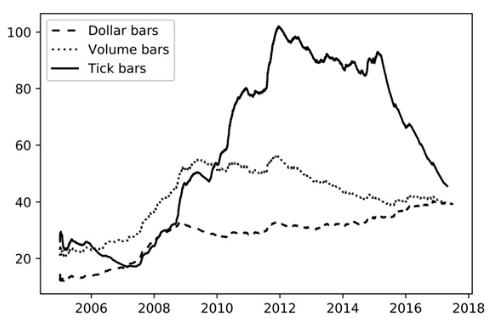
\includegraphics[scale=0.4]{/intro/standardbars}
\caption{Average daily frequency of tick, volume, and dollar bars}
\end{figure}

\begin{remark} \hlt{Standard BARS}\\
Method to transform a series of observations arriving at irregular frequency into a homogeneous series derived from regular sampling.
\begin{enumerate}[label=\roman*.]
\setlength{\itemsep}{0pt}
\item Time Bars: obtained by sampling information at fixed intervals. Information collected includes timestamp, volume-weighted average price (VWAP), open price, close price, high price, low price, volume etc.\\
To be avoided as markets do not process information at constant time interval. Time bars oversample information in low-activity periods and under-sample information in high-activity periods. Time bars exhibit poor statistical properties, i.e., serial correlation, heteroscedasticity, non-normality of returns.
\item Tick Bars: sample variables extracted each time a pre-defined number of transactions take place. Allows synchronisation of sampling with a proxy of information arrival.\\
Sampling as a function of trading activity creates returns closer to IID Normal (\cite{Thierry_Helyette_2000}). When constructing tick bars, to be aware of outliers, as many exchanges carry out auction at open and at close; order book accumulates bids and offers without matching. Order fragmentation introduces some arbitrariness in number of ticks. Matching engine protocols may split one fill into multiple artificial partial fills as a matter of operational convenience.
\item Volume Bars: samples every time a pre-defined amount of security's units that have been exchanged.\\
Achieves better statistical properties than sampling tick bars.\\
Convenient artefact for studying market microstructure theories.
\item Dollar Bars: samples an observation every time a pre-defined market value is exchanged. Used when the analysis involves significant price fluctuations. Robust against corporate actions such as splits, reverse splits, issuance of new shares, buying back existing shares.\\
Bar size could be dynamically adjusted as a function of free-floating market cap of a company or outstanding amount of issued debt.
\end{enumerate}
\end{remark}

\begin{remark} \hlt{Information-Driven Bars}\\
Method to sample more frequently when new (micro-structural) information arrives to the market.
\begin{enumerate}[label=\roman*.]
\setlength{\itemsep}{0pt}
\item Tick Imbalance Bars: sample bars whenever tick imbalance exceeds expectations. To determine tick index $T$ such that accumulation of signed ticks exceeds a given threshold.\\
Let $\{(p_t, v_t)\}_{t=1, \ldots, T}$ be sequence of ticks where $p_t$ and $v_t$ is the price and volume associated with tick $t$. Let tick rule define a sequence $\{b_t\}_{t=1, \ldots, T}$ where
\begin{align}
b_t = 
\begin{cases}
b_{t-1} \ \ \ \text{if } \Delta p_t = 0 \\
\frac{\abs{\Delta p_t}}{\Delta p_t} \ \ \text{if } \Delta p_t \neq 0
\end{cases} \nonumber
\end{align}
The tick imbalance at time $T$ is defined as 
\begin{equation}
\theta_T = \sum\limits_{t=1}^T b_t \nonumber
\end{equation}
Compute expected value of $\theta_T$ at beginning of the bar,
\begin{equation}
E_0[\theta_T] = E_0 [T](P[b_t = 1] - P[b_t = -1]) = E_0 [T](2P[b_t = 1] - 1) \nonumber
\end{equation}
where $E_0[T]$ is expected size of tick bar, $P[b_t = 1]$ and $P[b_t = -1]$ is unconditional probability that a tick is classified as a buy and sell. In practice, $E_0[T]$ and $(2P[b_t = 1] - 1)$ may be estimated as an exponentially weighted moving average of $T$ and $b_t$ values from prior bars.\\
Define the tick imbalance bar (TIB) as a $T^{*}$ contiguous subset of ticks such that
\begin{equation}
T^{*} = \arg \min_T \{ \abs{\theta_T} \geq E_0 [T] \ \vert \ 2 P[b_t = 1] - 1 \} \nonumber
\end{equation}
where the size of expected imbalance is implied by $\abs{2 P[b_t = 1] - 1}$.\\
When $\theta_T$ is more imbalanced than expected, a low $T$ will satisfy the conditions.\\
TIBs are produced more frequently under presence of informed trading (asymmetric information that triggers one-side trading). TIBs are buckets of trades containing equal amounts of information.
\item Volume/Dollar Imbalance Bars: sample bars when volume or dollar imbalances diverge from expectations.
\end{enumerate}
\end{remark}
